\documentclass[a4paper, 12pt]{article}
\usepackage[utf8x]{inputenc}
\usepackage{cmap}
\usepackage[english, russian]{babel}
\usepackage{indentfirst}
\usepackage[left=20mm, top=20mm, right=20mm, bottom=20mm]{geometry}
\usepackage{tikz}
\usepackage{float}
\usepackage{amsmath, amsfonts, amssymb}
\usepackage{graphicx}
\usepackage{fancybox, fancyhdr}
\usepackage{hyperref}
\usepackage{listings}
\usepackage{caption}
\usepackage{subcaption}
\usepackage{xcolor}
\pagestyle{fancy}
\fancyhf{}
\fancyhead[L]{Домашнее задание №2}
\fancyhead[R]{Теоретическая вероятность}
\fancyfoot[C]{\thepage}
\graphicspath{{images/}}
\usetikzlibrary{patterns}
\definecolor{LightGray}{gray}{0.95}
\definecolor{LightGray2}{gray}{0.7}
\lstdefinestyle{pycode}{
    language=Python,
    basicstyle=\footnotesize\ttfamily,
    numbers=left,
    numberstyle=\scriptsize\color{gray},
    stepnumber=1,
    numbersep=5pt,
    backgroundcolor=\color{LightGray},
    showspaces=false,
    showstringspaces=false,
    showtabs=false,
    tabsize=4,
    captionpos=b,
    breaklines=true,
    breakatwhitespace=false,
    frame=single,
    rulecolor=\color{LightGray2},
    linewidth=\linewidth,
    keywordstyle=\color{blue}\bfseries,
    commentstyle=\color{green!40!black},
    stringstyle=\color{purple},
    escapeinside={\%*}{*)},
    inputencoding=utf8x,
    xleftmargin=0pt,
    framexleftmargin=0pt,
    framexrightmargin=0pt
}
\lstset{style=pycode}
\hypersetup{
    colorlinks=true,
    linkcolor=blue,
    filecolor=magenta,
    urlcolor=cyan,
    pdftitle={contents setup},
    pdfpagemode=FullScreen,
}
\setlength{\parskip}{1.5mm}
\setlength{\headheight}{15pt}
\setlength{\footskip}{15pt}
\allowdisplaybreaks
\DeclareMathOperator{\sinc}{sinc}
\newcommand{\frc}[2]{\raisebox{2pt}{$#1$}\big/\raisebox{-3pt}{$#2$}}

\begin{document}
    \begin{titlepage}

        \begin{center}
        
\includegraphics[width=0.3\textwidth]{itmo.png} % requires itmo.png in /images folder
        \vfill

        Федеральное государственное автономное образовательное учреждение высшего образования
        «Национальный Исследовательский Университет ИТМО»\\

        \vfill
        {\large\bf ДОМАШНЕЕ ЗАДАНИЕ №2}\\
        {\large\bf ПРЕДМЕТ «ТЕОРЕТИЧЕСКАЯ ВЕРОЯТНОСТЬ»}\\
        Вариант №1
        \vfill

        \begin{flushright}
            \begin{minipage}{.45\textwidth}
            {
                \hbox{Преподаватель:}
                \hbox{Шиманская Г. С.}
                \hbox{Студент:}
                \hbox{Румянцев А. А.}
                \hbox{}
                \hbox{Номер ИСУ:}
                \hbox{368731}
                \hbox{Поток:}
                \hbox{ТеорВер 1.2}
                \hbox{Факультет:}
                \hbox{СУиР}
                \hbox{Группа:}
                \hbox{R3241}
            }
            \end{minipage}
        \end{flushright}

        \vfill

        Санкт-Петербург\\
        2024
        \end{center}
    \end{titlepage}

    \tableofcontents

    \newpage
    \section{Задание 1.}
    \subsection{Условие задачи.}
    В кармане имеется 3 монеты по 5 рублей, 2 монеты по 3 рубля и 6 монет 
    по рублю. Из кармана случайным образом извлекаются три монеты, 
    составить ряд распределения суммы вытащенных из кармана денег, 
    построить функцию распределения, найти мат. ожидание, дисперсию, 
    с.кв.откл., медиану, моду. Построить график функции распределения, 
    многоугольник распределения.


    \subsection{Решение.}
    Рассмотрим различные комбинации трех монет. Пока что не будем учитывать перестановки.
    $$
    555,\ 553,\ 551,\ 331,\ 111,\ 531,\ 533,\ 311,\ 511
    $$
    Запомним соответствующие им суммы.
    $$
    15,\ 13,\ 11,\ 7,\ 3,\ 9,\ 11,\ 5,\ 7
    $$


    Числа в каждой из комбинаций можно располагать в разном порядке. Например, пятерки
    и единицы можно расположить в строку из трех чисел шестью способами. Поэтому нам
    потребуется использовать формулу сочетаний из $n$ по $k$ вида
    $$
    C_n^k=\dfrac{n!}{(n-k)!\,k!};
    $$
    Распишем число сочетаний для каждой из комбинаций, приведенных ранее.
    $$
    C_3^3,\ C_3^2\cdot C_2^1,\ C_3^2\cdot C_6^1,\ C_2^2\cdot C_6^1,\ C_6^3,\ C_3^1\cdot C_2^1\cdot C_6^1,\ C_3^1\cdot C_2^2,\ C_2^1\cdot C_6^2,\ C_3^1\cdot C_6^2
    $$


    Чтобы найти вероятность с помощью перестановок нужно учесть все возможные исходы. Всего монет 11,
    а берем мы 3, значит для нахождения вероятности нам потребуется поделить число сочетаний для каждого
    рассматриваемого случая на
    $$
    C_{11}^3=\dfrac{11!}{(11-3)!\,3!}=165;
    $$
    Пример расчета приведен ниже.
    $$
    \dfrac{C_3^1\cdot C_2^1\cdot C_6^1}{C_{11}^3}=\dfrac{\dfrac{3!}{2!}\cdot\dfrac{2!}{1!}\cdot\dfrac{6!}{5!}}{165}=\dfrac{12}{55}
    $$


    Теперь составим ряд распределения суммы вытащенных из кармана денег.
    Ранее мы записывали ее для каждой из комбинаций. Видим, что сумма в 7 и 11 рублей повторяются дважды --
    вероятность для этих сумм будет складываться из соответствующих вероятностей, посчитанных формулой сочетаний.
    Получим следующее:
    $$
    P(X=7)=\dfrac{C_2^2\cdot C_6^1}{C_{11}^3}+\dfrac{C_3^1\cdot C_6^2}{C_{11}^3}=\dfrac{2}{55}+\dfrac{3}{11}=\dfrac{17}{55}
    $$
    $$
    P(X=11)=\dfrac{C_3^2\cdot C_6^1}{C_{11}^3}+\dfrac{C_3^1\cdot C_2^2}{C_{11}^3}=\dfrac{6}{55}+\dfrac{1}{55}=\dfrac{7}{55}
    $$


    \newpage
    Теперь составим таблицу $p_i(x_i)$.
    \begin{table}[h]
        \centering
        \begin{tabular}{|c|c|c|c|c|c|c|c|}
        \hline
        $x_i$ & 3 & 5 & 7 & 9 & 11 & 13 & 15 \\
        \hline
        $p_i$ & $\frc{4}{33}$ & $\frc{2}{11}$ & $\frc{17}{55}$ & $\frc{12}{55}$ & $\frc{7}{55}$ & $\frc{2}{55}$ & $\frc{1}{165}$ \\
        \hline
        \end{tabular}
        \caption{Ряд распределения суммы вытащенных из кармана денег.}
        \label{tab:moneysum}
    \end{table}


    Запишем функцию распределения $F(x)$, построим ее график и многоугольник распределения.
    $$F(x)=
    \begin{cases}
        0, & x\leq 3\\
        \frc{4}{33}, & 3 < x \leq 5\\
        \frc{10}{33}, & 5 < x \leq 7\\
        \frc{101}{165}, & 7 < x \leq 9\\
        \frc{137}{165}, & 9 < x \leq 11\\
        \frc{158}{165}, & 11 < x \leq 13\\
        \frc{164}{165}, & 13 < x \leq 15\\
        1, & x > 15
    \end{cases}
    $$
    \begin{figure}[H]
        \centering
        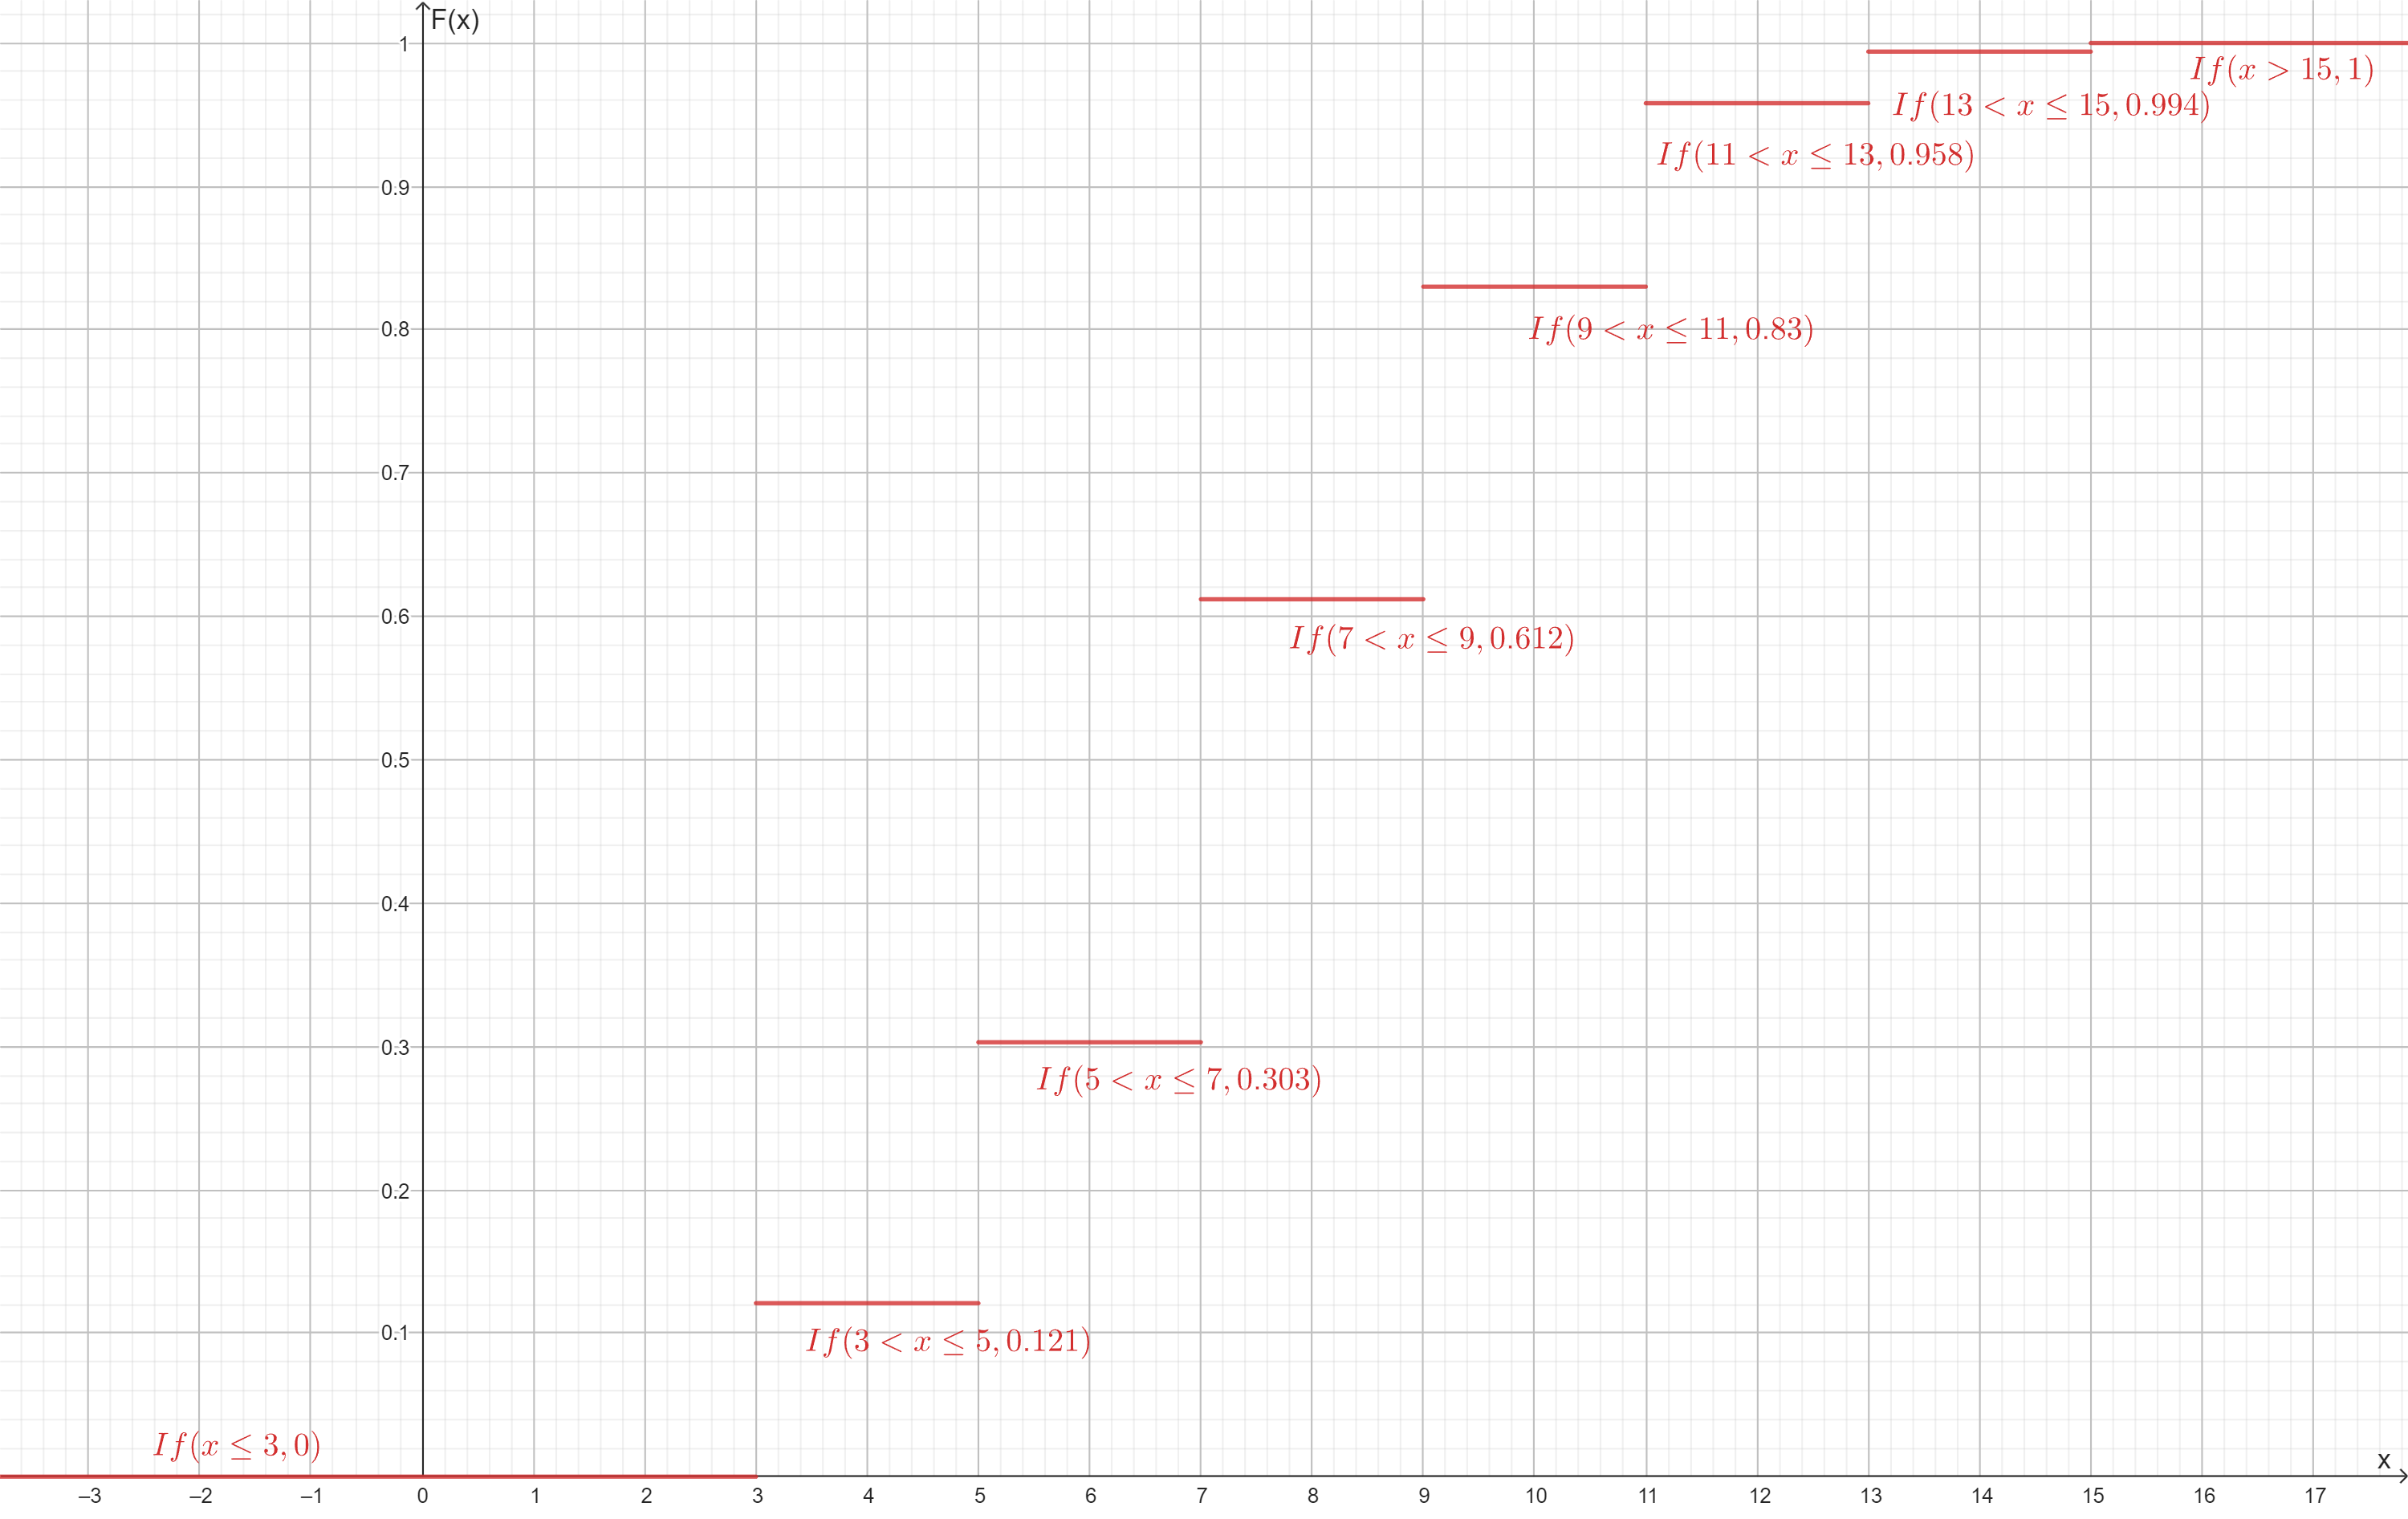
\includegraphics[scale=0.5]{F_x.png}
        \captionsetup{skip=0pt}
        \caption{График функции распределения.}
        \label{fig:F_x}
    \end{figure}
    \begin{figure}[H]
        \centering
        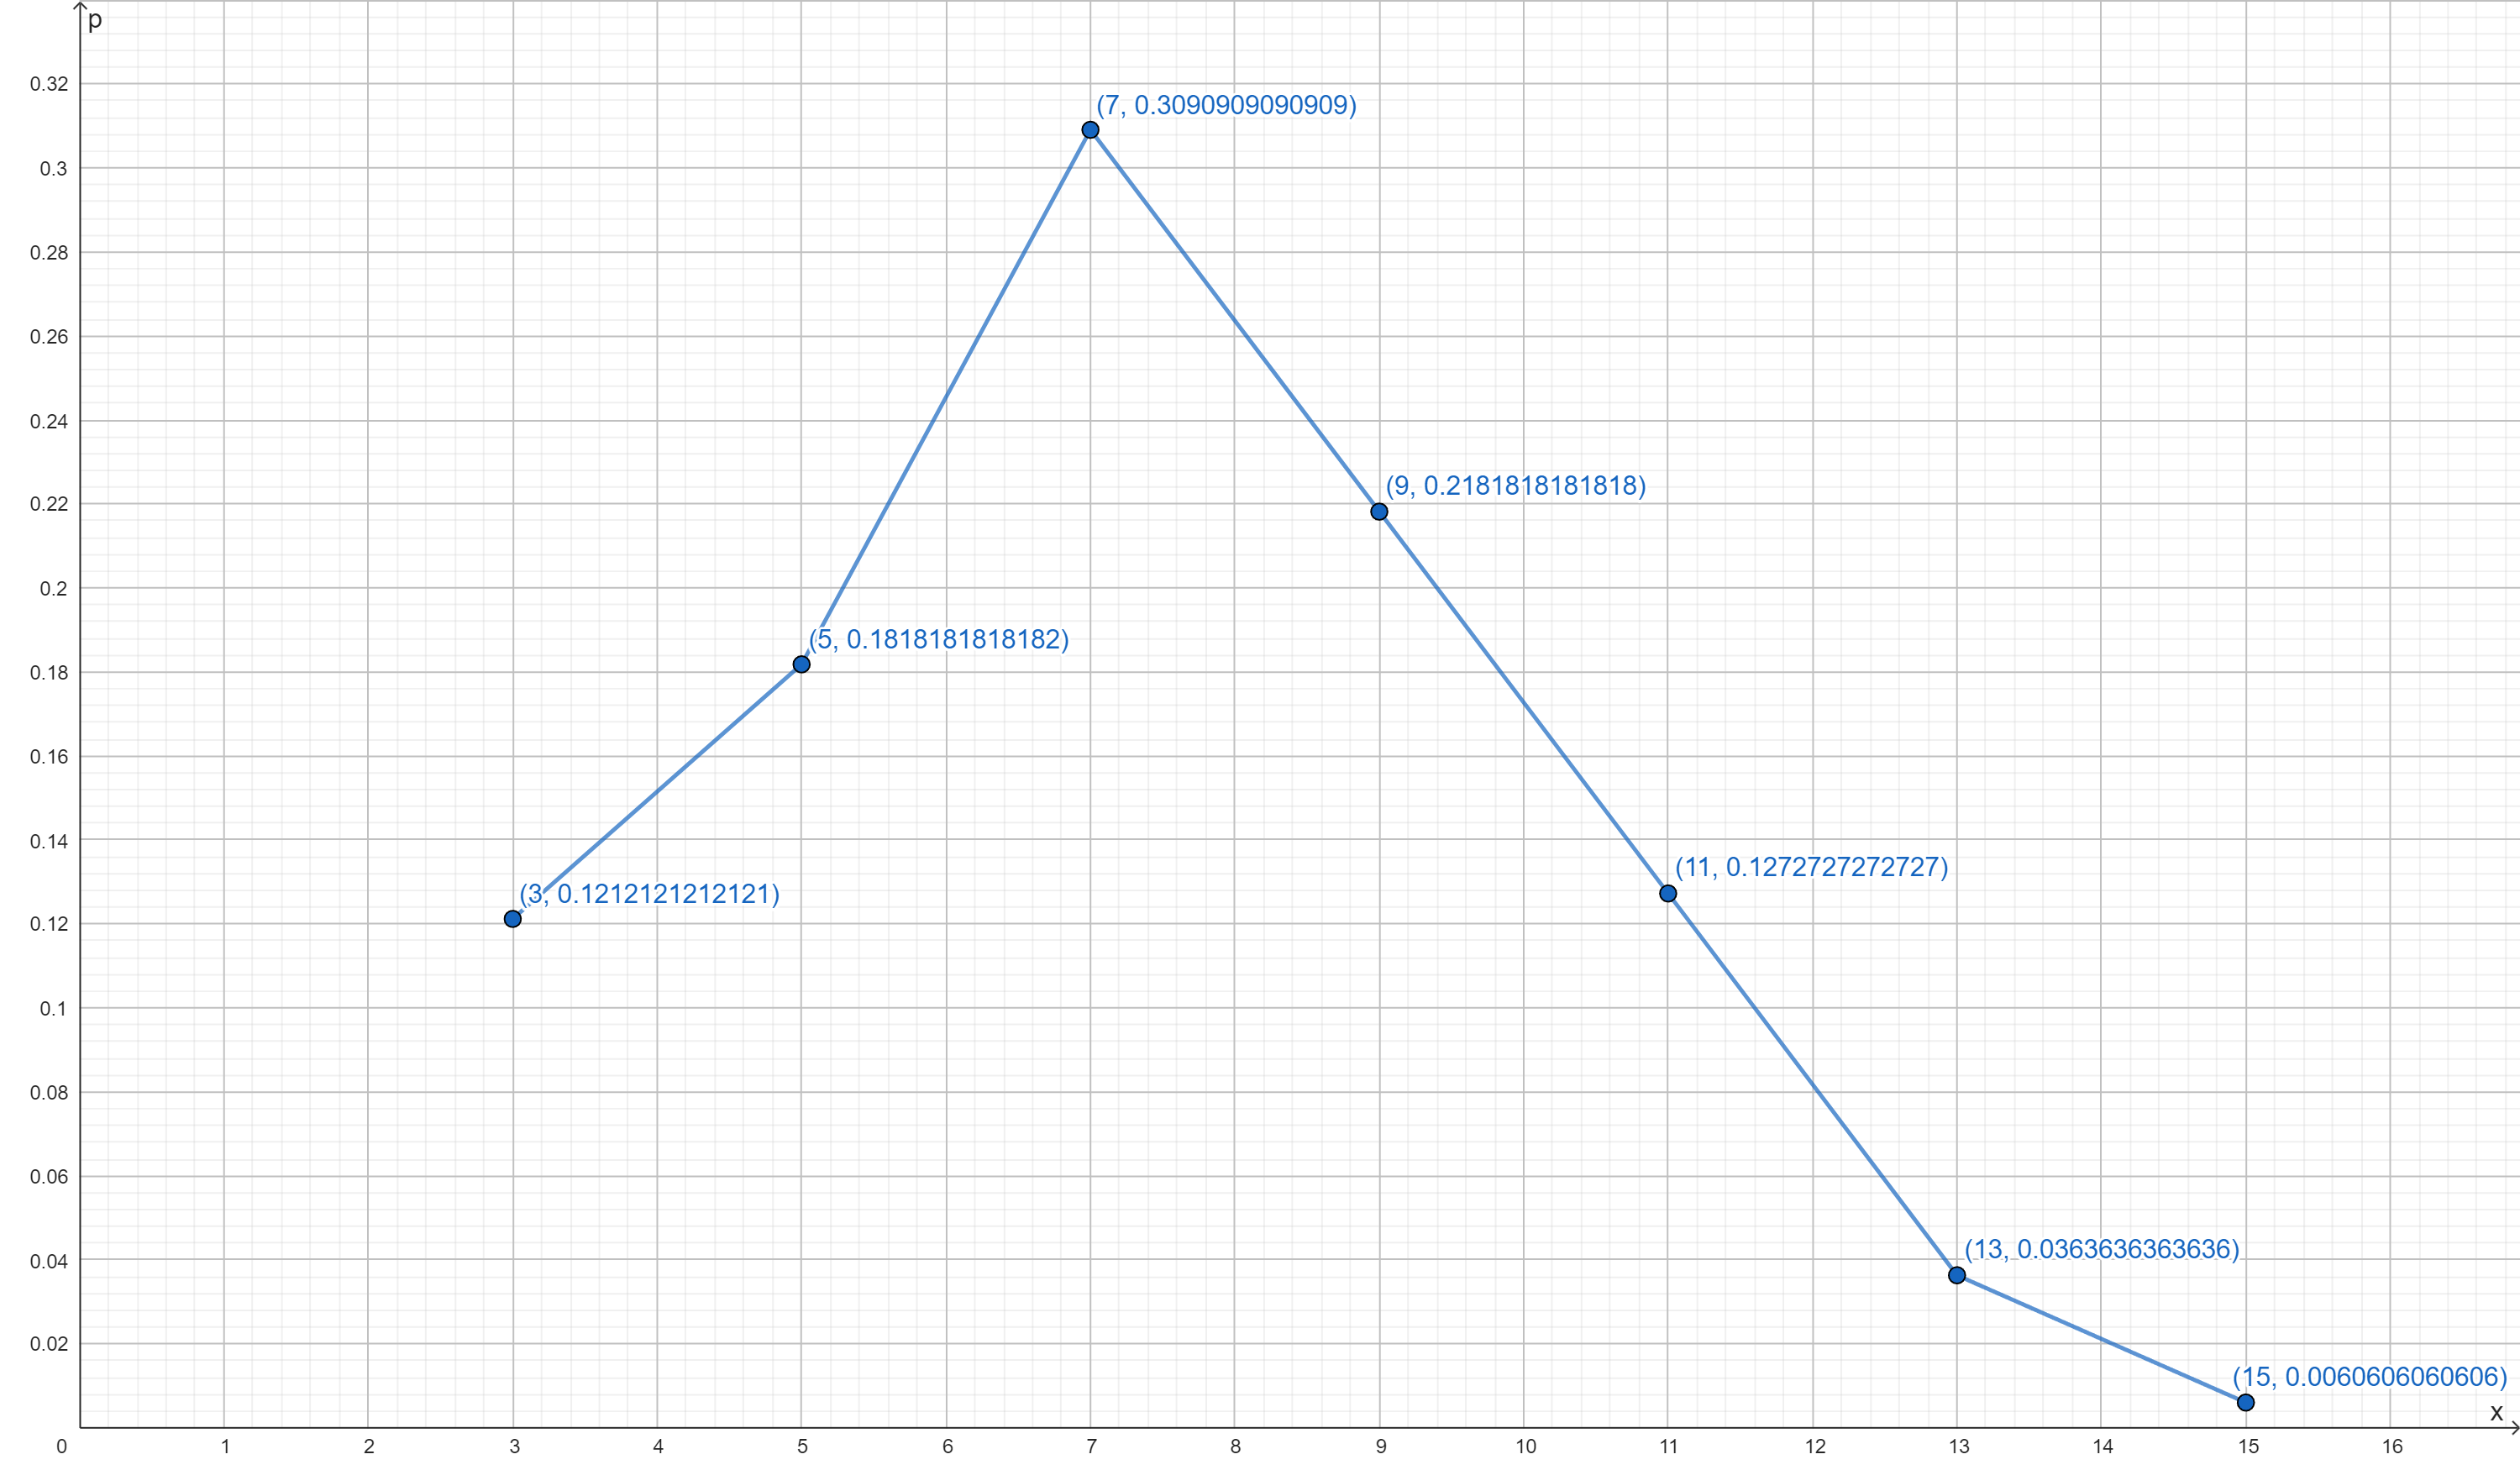
\includegraphics[scale=0.65]{polydis.png}
        \captionsetup{skip=0pt}
        \caption{Многоугольник распределения.}
        \label{fig:polydis}
    \end{figure}


    \newpage
    Далее найдем математическое ожидание ($k$ -- количество $x_i$), дисперсию, среднеквадратичное отклонение, медиану, моду и вероятность того,
    что сумма окажется не менее 10 рублей. Медиана -- средний элемент выборки, левее и правее которого одинаковое количество элементов,
    если в выборке нечетное количество значений. Мода -- самый часто повторяющийся элемент выборки. В нашем случае их два, поэтому я приведу оба.
    $$
    M(x)=\sum\limits_{i=1}^kx_ip_i=3\cdot\dfrac{4}{33}+5\cdot\dfrac{2}{11}+7\cdot\dfrac{17}{55}+9\cdot\dfrac{12}{55}+11\cdot\dfrac{7}{55}+13\cdot\dfrac{2}{55}+15\cdot\dfrac{1}{165}=\dfrac{81}{11},
    $$
    $$
    M(x^2)=\sum\limits_{i=1}^kx_i^2p_i=3^2\cdot\dfrac{4}{33}+5^2\cdot\dfrac{2}{11}+7^2\cdot\dfrac{17}{55}+9^2\cdot\dfrac{12}{55}+11^2\cdot\dfrac{7}{55}+13^2\cdot\dfrac{2}{55}+15^2\cdot\dfrac{1}{165}=\dfrac{675}{11},
    $$
    $$
    D(x)=M(x^2)-(M(x))^2=\dfrac{675}{11}-\left(\dfrac{81}{11}\right)^2=\dfrac{675}{11}-\dfrac{6561}{121}=\dfrac{864}{121},
    $$
    $$
    \delta(x)=\sqrt{D(x)}=\sqrt{\dfrac{864}{121}}=\dfrac{12\sqrt{6}}{11},
    $$
    $$
    MED(x)=9\Rightarrow P(X=MED(x)=9)=\dfrac{12}{55},
    $$
    $$
    MODE_1(x)=7\Rightarrow P(X=MODE_1(x)=7)=\dfrac{17}{55},
    $$
    $$
    MODE_2(x)=11\Rightarrow P(X=MODE_2(x)=11)=\dfrac{7}{55},
    $$
    $$
    P(X\geq 10)=P(X=11)+P(X=13)+P(X=15)=\dfrac{7}{55}+\dfrac{2}{55}+\dfrac{1}{165}=\dfrac{28}{165}
    $$


    \begin{align*}
        & \textbf{Ответ:}\\
        & \mathbf{M(X)=\dfrac{81}{11},\ D(X)=\dfrac{864}{121},\ \delta(X)=\dfrac{12\sqrt{6}}{11}}, \ \mathbf{P(X=MED(x)=9)=\dfrac{12}{55}}, \\
        & \mathbf{P(X=MODE_1(x)=7)=\dfrac{17}{55},\ P(X=MODE_2(x)=11)=\dfrac{7}{55},}\\ & \mathbf{P(X\geq 10)=\dfrac{28}{165}}
    \end{align*}


    \section{Задание 2.}
    \subsection{Условие задачи.}
    На рынок поступила партия арбузов. Предполагается, что вес одного 
    арбуза -- случайная величина, подчиняющаяся нормальному закону 
    распределения с математическим ожиданием $M(X) = 9$ кг и средним 
    квадратическим отклонением $\sigma = 0.5$ кг. Определите вероятность того, 
    что вес случайно отобранного арбуза:
    \begin{enumerate}
        \item Окажется больше 12 кг;
        \item Окажется меньше 7.5 кг;
        \item Будет находиться между 8.5 и 9.5 кг;
        \item Отклонится от математического ожидания меньше, чем на 0.1 кг;
        \item Отклонится от математического ожидания больше, чем на 0.2 кг;
    \end{enumerate}
    Найдите границы, в которых отклонение веса случайно отобранной 
    туши от своего математического ожидания не превысит утроенного среднего 
    квадратического отклонения (проиллюстрируйте правило трех сигм).


    \subsection{Решение.}
\end{document}